\section{Redes de Sensores Sem Fio}
\cite{Silva2009}
Com a queda crescente nos custos dos equipamentos eletrônicos, a redução no tamanho dos dispositivos simplificando a sua mobilidade, fez com que as redes sem fio ganhassem popularidade rapidamente mundo afora, ganhando novos tipos de aplicações com objetivo de simplificar o dia-a-dia das pessoas, como previsto por Weiser em \cite{Weiser1991}. 

Atualmente, a variedade de sensores\cite{SensoresXXXX} existentes e que podem ser obtidos sem muita dificuldade pela internet tem crescido exponencialmente. Aliado à uma consciência dos benefícios que a interligação desses dispositivos em rede para análise em tempo real das informações ambientais, geralmente invisíveis a nossa atenção no curto prazo \cite{Weiser:1997:CAC:504928.504934} podem oferecer ao dia-a-dia, faz da rede de sensores sem fio um dos pilares de sustentação da Internet das Coisas (IoT).

Decisões sobre a arquitetura, modelo e equipamentos utilizados em uma Redes de Sensores Sem Fio \cite{LECKER2010} (RSSF ou WSN) se tornaram fator de sucesso para projetos de IoT.

\begin{figure}[tbh!]
	\centering
	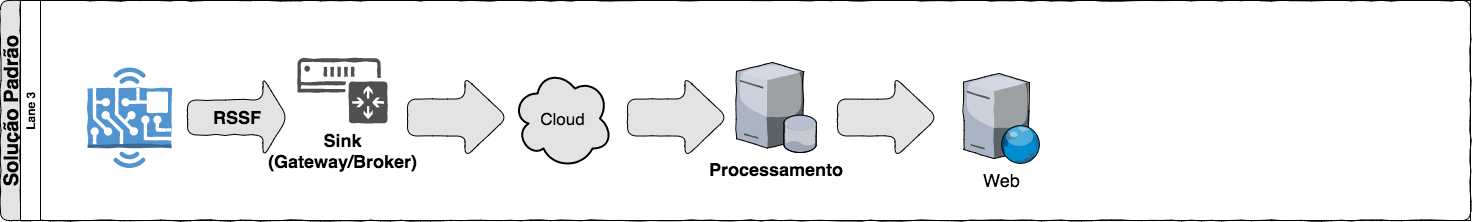
\includegraphics[width=1.0\textwidth]{../images/padrao_rede}
	\caption{Arquitetura RSSF padrão}
	\label{fig:rssfpadrao}
\end{figure}

Em \cite{Ueyama002840382} e \cite{Furquim002744726}, uma estrutura de sensores do tipo b\'{o}ia foi criada para coleta e análise do nível da água e sua poluição em rios.

\begin{figure}[tbh!]
	\centering
	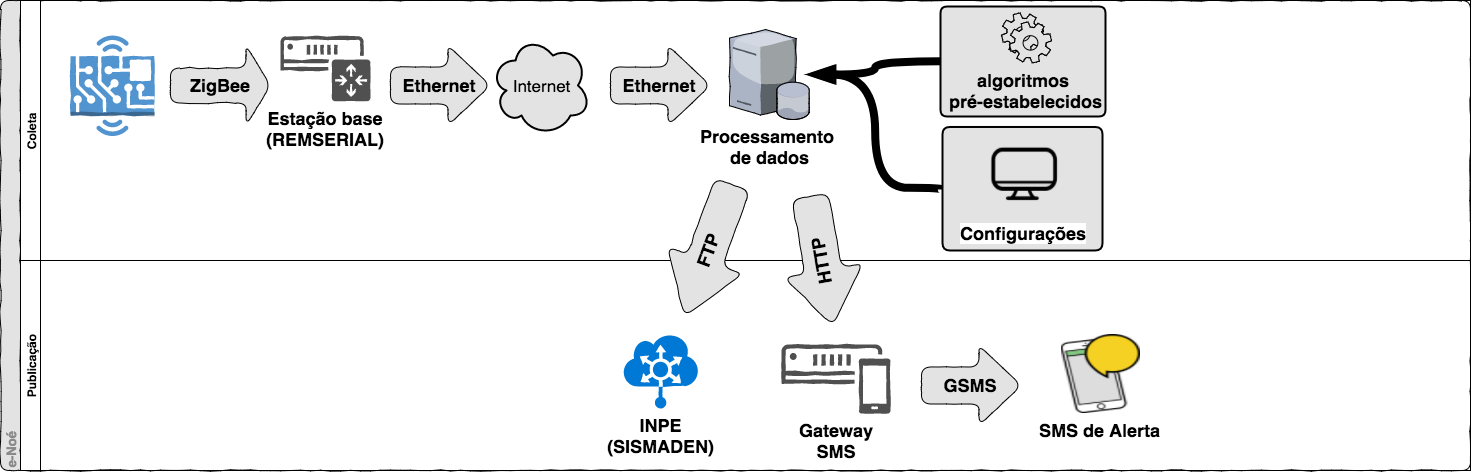
\includegraphics[width=1.0\textwidth]{../images/enoe_rede}
	\caption{Projeto e-Noé}
	\label{fig:enoe}
\end{figure}

De acordo com o trabalho realizado em \cite{Chen2014}, podemos analisar, classificar e quantificar os insetos encontrados em uma determinada região utilizando sensores acústicos, de forma a utilizar os resultados encontrados para aplicação de uma quantidade determinada de defencivos, controlando o efeito de sua aplicação em tempo real.

Para se criar um modelo automatizado para controle do uso de recursos com custos reduzidos de forma a gerar menor impacto financeiro aos agricultores familiares é imprecindivel se  

Na prática seria usar RSSF, sensores, atuadores e um sistemas distribuído para automatizar processos como o de gotejamento localizado como descrito nas imagens abaixo, baseado em informações retiradas da bdpa (base de pesquisas agropecuária) da embrapa.


\section{Ontologias}

\section{Modelagem dos Dados}

\section{Social Virtual Objects}

\section{Identifica\c{c}\~{a}o dos objetos na rede}
	Embora seja relativamente novo, o dom\'{i}nio de Internet das Coisas tem sido alvo de pesquisas h\'{a} algum tempo. Universidades, empresas e organiza\c{c}\~{o}es t\^{e}m empregado esfor\c{c}os para definir, propor e implementar solu\c{c}\~{o}es que prover\~{a}o suporte para essa nova \'{a}rea que tende a se popularizar nos pr\'{o}ximos anos.	
	
\subsection{Agrupamento de objetos por Federa\c{c}\~{o}es}
	 A infraestrutura baseada em federa\c{c}\~{a}o (IOT-A, 2011) consiste em uma arquitetura proposta com base em conceitos apresentados em (MCLEOD e HEIMBIGNER, 1980) e busca tratar a heterogeneidade de cena?rios e recursos sem exigir uma abordagem que force uma solu\c{c}\~{a}o u?nica para a resolu\c{c}\~{a}o de nomes. Nessa arquitetura, propo?e-se que cada n\'{o} represente um local que agregue diversos recursos e	

\subsection{Agrupamento de objetos utilizando RNS}
	Algumas abordagens, como o RNS, proposto em (TIAN et al, 20012), buscam manter a compatibilidade com os sistemas de Internet das Coisas j\'{a} existentes. Projetado para ser uma plataforma capaz de suportar sistemas de nomea\c{c}\~{a}o e resolu\c{c}\~{a}o distintos, o RNS busca n\~{a}o exigir altera\c{c}\~{o}es significativas nos sistemas j\'{a} criados.


\section{Sinks e algoritmos de coleta de dados}

